\section{Recursive running time analysis}

\paragraph*{Merge sort}
One possible recursive solution to the sorting problem is the merge sort algorithm, that takes as input an array $A[n]$.  
\begin{algorithm}[H]
    \caption{Merge sort}
        \begin{algorithmic}[1]
            \If {$n=1$}
                \State\Return $A[n]$
            \EndIf
            \State Recursively sort the two half lists $A\left[1\ldots\left\lceil \frac{n}{2}\right\rceil \right]$ and $A\left[\left\lceil \frac{n}{2}\right\rceil + 1 \ldots n\right]$
            \State Merge ($A\left[1\ldots\left\lceil \frac{n}{2}\right\rceil \right]$, $A\left[\left\lceil \frac{n}{2}\right\rceil + 1 \ldots n\right]$)
        \end{algorithmic}
\end{algorithm}
The key subroutine of the given algorithm is merge, that makes the algorithm recursive. 

For the complexity analysis we have to consider the following elements: 
\begin{itemize}
    \item If the array contains only one element (first line), the complexity is constant, resulting in $\Theta(1)$. 
    \item The recursive sort of the two lists (line four) cost a total of $(\left\lceil \frac{n}{2} \right\rceil+\left\lfloor \frac{n}{2} \right\rfloor )$, but since floor and ceiling does not matter asymptotically we have a total complexity of $2T\left(\frac{n}{2}\right)$. 
        This is because the complexity of this sorting depends on the complexity of the algorithm itself. 
    \item Finally, the merging of the lists has a linear cost, since we need to check all the elements in the lists, yielding a complexity of $\Theta(n)$. 
\end{itemize}
The final result for the merge sort algorithm is: 
\[t(n)=\begin{cases}
    \Theta(1)\qquad\qquad\qquad\: \text{ if }n=1 \\
    2T\left(\frac{n}{2}\right) + \Theta(n)\qquad\:\text{if }n>1
\end{cases}\]
In case in which the base case has a complexity of $\Theta(1)$ for sufficiently small $n$ we can omit it. 
However, this can be done only when it has no effect on the asymptotic solution to the recurrence. 

\subsection{Recursion tree}
To find the complexity of the merge sort algorithm we need to solve the equation: 
\[T(n)=2T\left(\frac{n}{2}\right)+c\cdot n\]
To do so we can use the recursion tree, starting from the root. 
We continue to expand the leaf until we cannot go further down because we reached the base case. 
For this algorithm a partial recursion tree is the following: 
\begin{figure}[H]
    \centering
    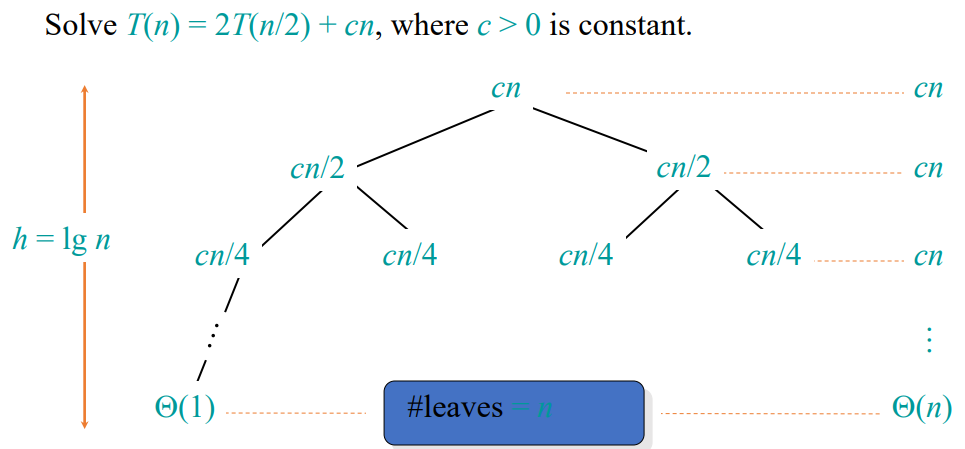
\includegraphics[width=0.75\linewidth]{images/tree.png}
    \caption{Partial recursion tree for merge sort algorithm}
\end{figure}

At this point we have a depth of $h=\log_2(n)$, and a total of $n$ leaves. 
As a result, the algorithm's complexity is the product of number of leaves with the depth of the tree, that is: 
\[T(n)=\Theta(\log_2(n)\cdot n)\]

The final result shows that $\Theta(\log_2(n)\cdot n)$ grows more slowly than $\Theta(n^2)$. 
Therefore, merge sort asymptotically beats insertion sort in the worst case.
In practice, merge sort beats insertion sort for $n > 30$ or so.

\subsection{Substitution method}
The substitution method is the most general method to solve recursive complexity equations.
The steps to apply the substitution method are: 
\begin{enumerate}
    \item Guess the form of the solution by performing a preliminary analysis on the algorithm. 
    \item Verify by induction. 
    \item Solve for constants. 
\end{enumerate}
\begin{example}
    Consider the following expression: 
    \[T(n)=4T\left(\frac{n}{2}\right)+n\]
    We assume that the base case is $T(1)=\Theta(1)$. 
    We can now apply the substitution method with by performing the following steps: 
    \begin{enumerate}
        \item We guess that the solution has a complexity of $O(n^3)$, ad so we assume that $T(k)\leq c\cdot k^3$ for $k<n$. 
        \item We verify by induction that $T(n)\leq c\cdot n^3$. 
    \end{enumerate}
\end{example}
The problem with this approach is that it is not simple to apply in every situation. 

\subsection{Master method}
To overcome the complexity of the substitution method we may use the master method. 
The master method applies to recurrences of the form: 
\[T(n)=aT\left(\frac{n}{b}\right)+f(n)\]
Here, $a\geq 1$, $b>1$, and $f(n)$ is asymptotically positive. 
So, it is less general than substitution, but it is more straightforward. 

In general, this method is always applicable for divide and conquer style algorithms. 

To apply this method we have to compare $f(n)$ with $n^{\log_ba}$. 
We could have three outcomes: 
\begin{enumerate}
    \item $f(n)=O(n^{\log_ba-\varepsilon})$ for some constant $\varepsilon > 0$. 
        In this case we have that the function $f(n)$ grows polynomially slower than $n^{\log_ba}$ by an $n^\varepsilon$ factor. 
        In this scenario the solution is: 
        \[T(n)=\Theta(n^{\log_ba})\]
    \item $f(n)=\Theta(n^{\log_ba}\log^kn)$ for some constant $k \geq 0$. 
        In this case we have that the function $f(n)$ and $n^{\log_ba}$ grow at similar rates. 
        In this scenario the solution is: 
        \[T(n)=\Theta(n^{\log_ba}\log^{k+1}n)\]
    \item $f(n)=\Omega(n^{\log_ba+\varepsilon})$ for some constant $\varepsilon > 0$. 
        In this case we have that the function $f(n)$ grows polynomially faster than $n^{\log_ba}$ by an $n^\varepsilon$ factor, and $f(n)$ satisfies the regularity condition that $a \cdot f\left(\frac{n}{b}\right) \leq c \cdot f(n)$ for some constant $c < 1$.
        In this scenario the solution is: 
        \[T(n)=\Theta(f(n))\]
\end{enumerate}
\begin{example}
    Let's consider the expression: 
    \[T(n)=4T\left(\frac{n}{2}\right)+n\]
    In this expression we have that $a=4$ and $b=2$, so we have that: 
    \[n^{\log_ba}=n^2 \qquad f(n)=n\]
    So we have are in the first case of the theorem, that is $f(n)=O(n^{2-\varepsilon})$ for $\varepsilon=1$. 
    So, the solution is: 
    \[T(n)=\Theta(n^2)\]

    Let's consider the expression: 
    \[T(n)=4T\left(\frac{n}{2}\right)+n^2\]
    In this expression we have that $a=4$ and $b=2$, so we have that: 
    \[n^{\log_ba}=n^2 \qquad f(n)=n^2\]
    So we have are in the second case of the theorem, that is $f(n)=\Theta(n^2\log^kn)$ for $k=0$. 
    So, the solution is: 
    \[T(n)=\Theta(n^2\log n)\]

    Let's consider the expression: 
    \[T(n)=4T\left(\frac{n}{2}\right)+n^3\]
    In this expression we have that $a=4$ and $b=2$, so we have that: 
    \[n^{\log_ba}=n^2 \qquad f(n)=n^3\]
    So we have are in the second case of the theorem, that is $f(n)=\Omega(n^{2+\varepsilon})$ for $\varepsilon=1$. 
    So, the solution is: 
    \[T(n)=\Theta(n^3)\]

    Let's consider the expression: 
    \[T(n)=4T\left(\frac{n}{2}\right)+\frac{n^2}{\log n}\]
    In this expression we have that $a=4$ and $b=2$, so we have that: 
    \[n^{\log_ba}=n^2 \qquad f(n)=\frac{n^2}{\log n}\]
    In this case the method does not apply in this case. 
    In particular, for every constant $\varepsilon > 0$, we have $n^\varepsilon = \omega(\log n)$.
\end{example}